{\color{indiagreen}\subsection{Prožnostna energija}}
Delo pri raztezanju vzmeti.\\
\begin{align*}
	A &= \frac{kx^2}{2}\\
	A &= W_{pr}\\
	{\color{bostonuniversityred}W_{pr}} &= {\color{bostonuniversityred}\frac{kx^2}{2}}\\
	{\color{bostonuniversityred}\Delta W_{pr}} &= {\color{bostonuniversityred}\frac{kx_2^2}{2} - \frac{kx_1^2}{2}}\\
	0 &= \Delta W_k \Delta W_p\\
	{\color{bostonuniversityred}\Delta W_k \Delta W_p} &= konst. \text{Izrek o ohranitvi $W_k$ in $W_p$}\\
\end{align*} 
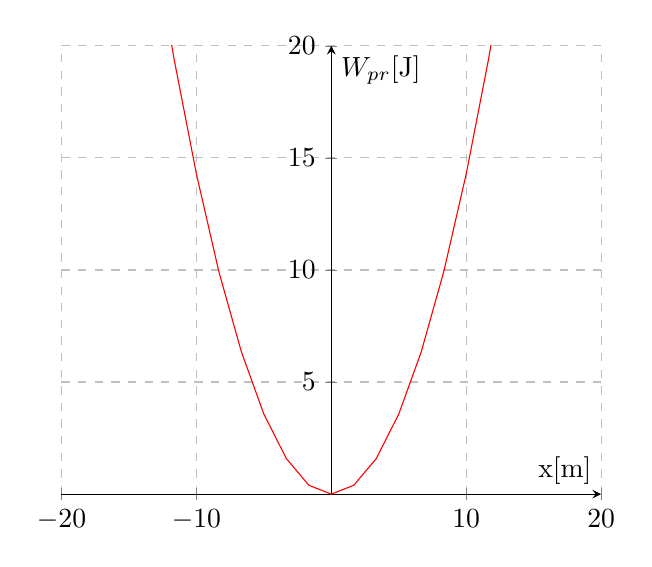
\begin{tikzpicture}
	\begin{axis}[
	    xlabel={x[m]},
	    ylabel={$W_{pr}$[J]},
	    xmin=-20, xmax=20,
	    ymin=0, ymax=20,
	    xtick={-20,-10,0,10,20},
	    ytick={0,5,10,15,20},
	    ymajorgrids=true,
	    xmajorgrids=true,
	    grid style=dashed,
	    axis lines=middle,
	]
	 
	\addplot[domain=-20:20,red] {x^2 / 7};

	\end{axis}
\end{tikzpicture}